% Section 2 of manuscript v0.2 (docs/paper/manuscript.md), converted without changes to claims or numbers.
\section{Hardware and recording setup}\label{sec:hardware}

\subsection{Plant and vessel}\label{sec:plant}

Camera 100 is installed at the Slovensk\'e cukrovary sugar plant in Sere\v{d}, Slovakia, on the \textbf{seed pan}:
the graining vacuum pan, designated ZRA in the plant control system (Slovak \emph{o\v{c}kovac\'i varostroj};
Slovensk\'e cukrovary plant Q\&A, 2026-08-12; DeltaV ``Udaje ZRA'' screen; \citealp{SlovenskeCukrovary2026};
English--Slovak glossary in Appendix~\ref{app:glossary}). The seed pan is seeded with milled-sugar slurry
(\emph{mikroo\v{c}ko}) and produces the seed massecuite (\emph{o\v{c}kovacia cukrovina}) that is dosed into the A
vacuum pans, where the product is boiled (operator A.~Fedor, pers.\ comm., 2026-11-03); the C stage is likewise
started from seed massecuite (plant Q\&A). The seed slurry's crystal-size distribution is independently characterised
by laser-diffraction granulometry (Mastersizer, 2-propanol dispersant; see \secref{sec:csd} preface and
\citealp{Mastersizer2025}) with $D[3;2] = 3.95$~\um, $D[4;3] = 8.71$~\um{} and
$\mathrm{Dv}(10) / \mathrm{Dv}(50) / \mathrm{Dv}(90) = 1.56 / 6.81 / 18.5$~\um. Vessel-level dimensions, agitation
regime, and operating temperature of the seed pan have not yet been independently audited and are deferred to a
follow-up revision; the camera-side hardware (\secref{sec:camera}) is operator-verified.

The seed pan is mechanically stirred (stirrer current tag EI1004) in normal operation, which is the physical basis on
which we invoke the homogeneous-slurry assumption of \secref{sec:homog}: the stirred massecuite continually refreshes
the slab actually imaged through the sight glass (\secref{sec:slab}), so the millimetre-thin slice is a
near-representative sample of the bulk population. A stage-specific audit of the recirculation rate vs.\ residence
time is on the follow-up list.

The camera observes the slurry through a circular borosilicate sight glass marked \code{DIN 8902}, mounted on an
8-bolt PN10 flange (\O150~mm / DN150, 20~mm thick, both measured on site 2026-09-07). The lens stack is horizontal,
with transmitted illumination from an LED inside the vessel on the opposite side of the slurry. Full hardware audit
and photographs are in the project's lens documentation (\code{docs/lens/README.md}).

\subsection{Camera and lens}\label{sec:camera}

The camera is a \textbf{Hanwha Vision HCB-6000}, an analogue HD box camera with a 1/2.8\,in progressive-scan CMOS
sensor (Sony IMX307/IMX327 die, identified from the datasheet total-pixel count $1945 \times 1097$;
$5.57 \times 3.13$~mm active area, $1920 \times 1080$~px, 2.9~\um{} pitch, 30~fps, AHD/TVI/CVI/CVBS-PAL output). The
lens is a \textbf{Fujinon HF35HA-1B}, a C-mount machine-vision lens with $f = 35$~mm, F-number range F/1.6 -- F/22,
image-format 2/3\,in (\O~11~mm circle), minimum object distance 0.25~m, back focal distance 15.03~mm in air, manual
iris with lock screws. Operator measurement on site (2026-06-15, corrected 2026-09-07) yielded an extension tube of
$\boldsymbol{e = 60}$~\textbf{mm} between the lens C-mount thread and the camera body, an F-number setting of
\textbf{F/1.6} (wide open), and a lens-front-to-glass air gap of $\boldsymbol{a = 20}$~\textbf{mm}. These numbers
together fix the working distance $d_\mathrm{focus} = 55.1$~mm and the scale 1.66~\umpx{} (\secref{sec:thinlens});
they are used throughout this paper.

\begin{quote}
\textbf{Revision note (2026-09-07).} Geometry and all detector outputs (CSD, KPI tables) in this manuscript were
rerun at the measured $e = 60$~mm / $t = 20$~mm / $a = 20$~mm. The dent-sharpness figure (\figref{fig:dents}) and
its $c = 5.8$~\um{} calibration predate the correction; its generating script is not in the repository.
\end{quote}

\subsection{Recording protocol and frame conditioning}\label{sec:recording}

The case-study video is \code{2026-02-05 10-36-32.mp4} (1568 frames, 30~fps, $1920 \times 1080$~px). The recording
carries \textbf{two distinct sources of frame contamination}, both of which inject artificially sharp edges that
overwhelm any per-pixel sharpness statistic computed on the raw frame (\secref{sec:empirical}):
\begin{enumerate}
\item \textbf{A burnt-in DVR overlay} --- a digital \code{YYYY-MM-DD HH:MM:SS} timestamp band in the top
${\sim}45$ rows and a \code{CH01} channel label in the bottom ${\sim}100$ rows. These are \emph{infinitely sharp
digital glyphs}.
\item \textbf{Analogue-aspect black bars} --- the leftmost ${\sim}40$ columns and the rightmost ${\sim}55$ columns
are pitch black (the analogue capture chain pads 4:3 source into a 16:9 frame). The transition between the black
bar and the live image produces a Laplacian$^2$ value of ${\sim}110$ (vs ${\sim}10$ for typical crystal-edge pixels)
--- an order of magnitude above any real signal.
\end{enumerate}

Both are removed by a single conservative frame crop: \code{CropBox(top=55, bottom=120, left=50, right=70)} from
\code{optics.video_io}. The cropped frame retains $1800 \times 905$~px $\approx 78$\,\% of the original frame area.
The crop box is one parameter; tune per recording if the DVR layout or analogue-aspect padding differs.

\figref{fig:frames} shows the raw and cropped first frame side by side. Every figure below uses the cropped variant.

\begin{figure}
\centering
\begin{subfigure}{\columnwidth}
\centering
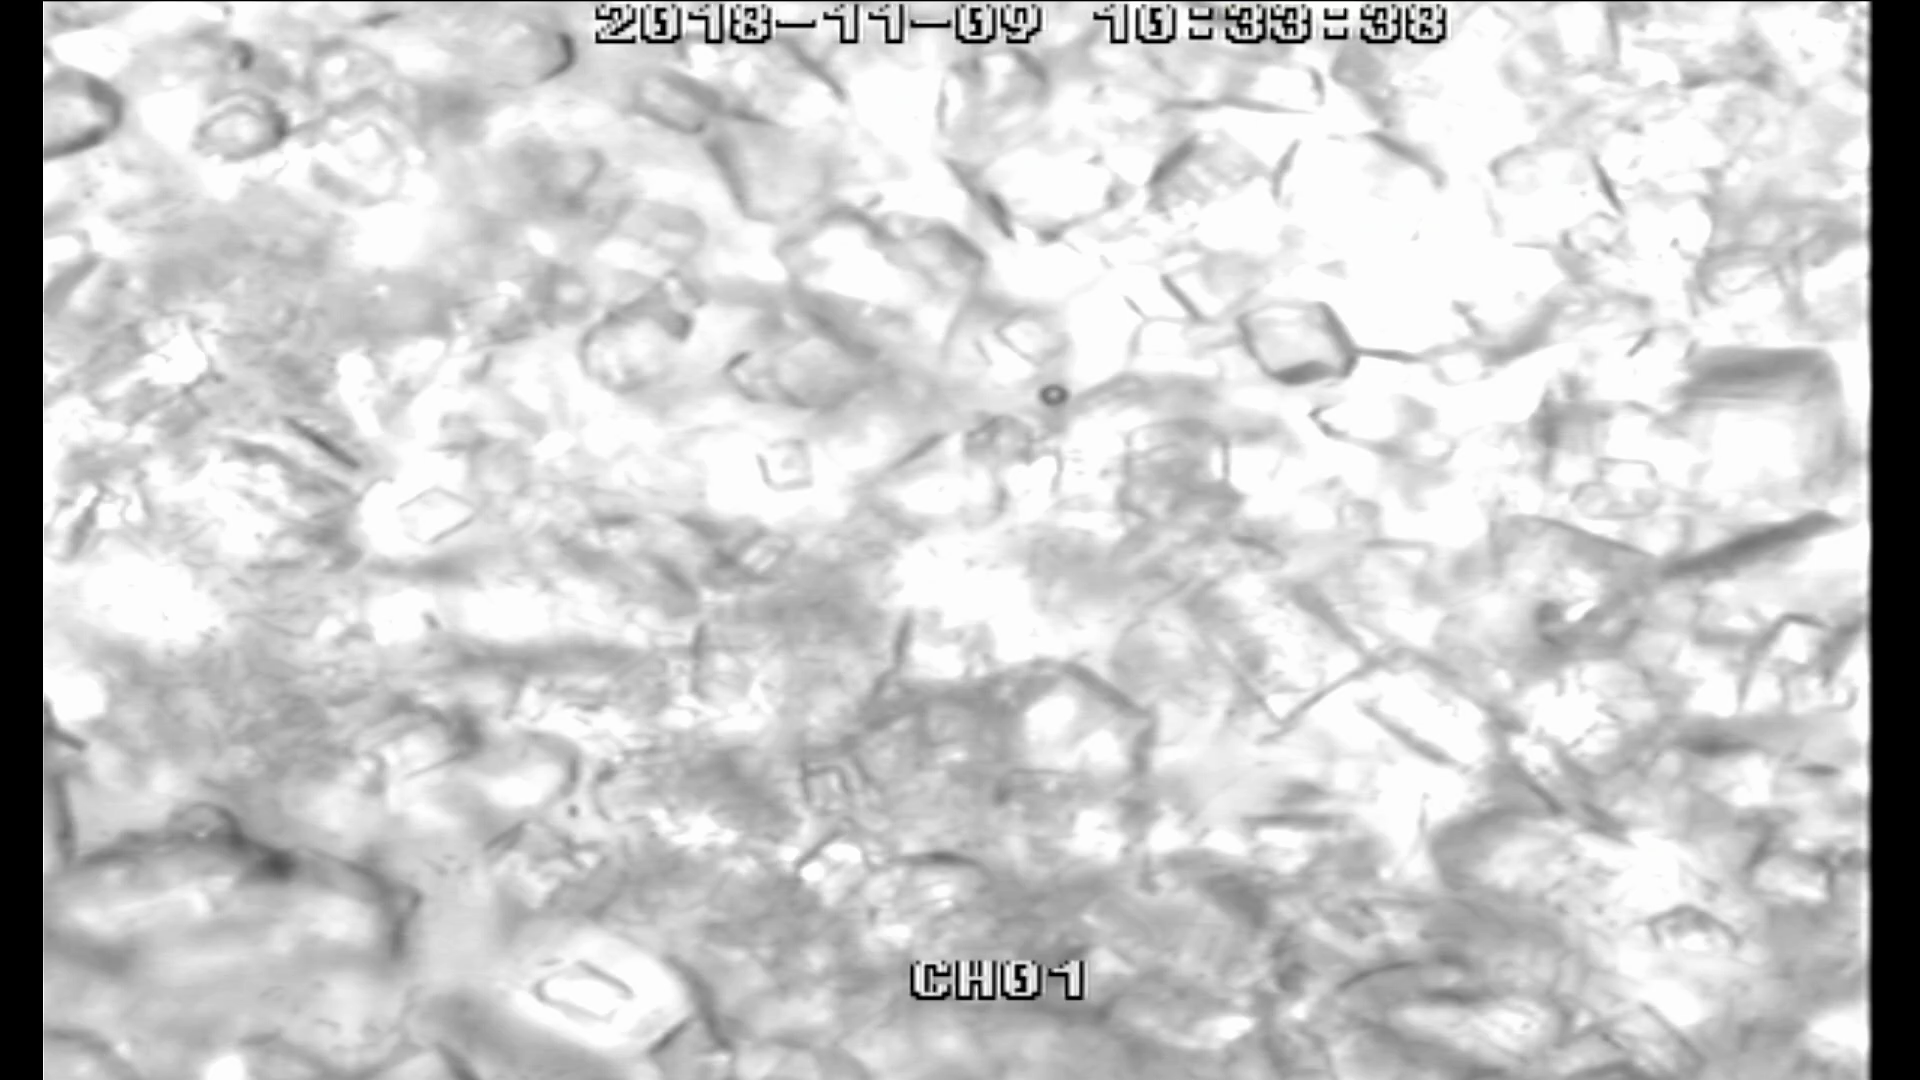
\includegraphics[width=\linewidth]{00_first_frame}
\caption{Raw first frame, $1920 \times 1080$. Top: DVR timestamp band. Bottom: \texttt{CH01} label. Left \& right:
analogue-aspect black bars.}\label{fig:frames-raw}
\end{subfigure}

\medskip
\begin{subfigure}{\columnwidth}
\centering
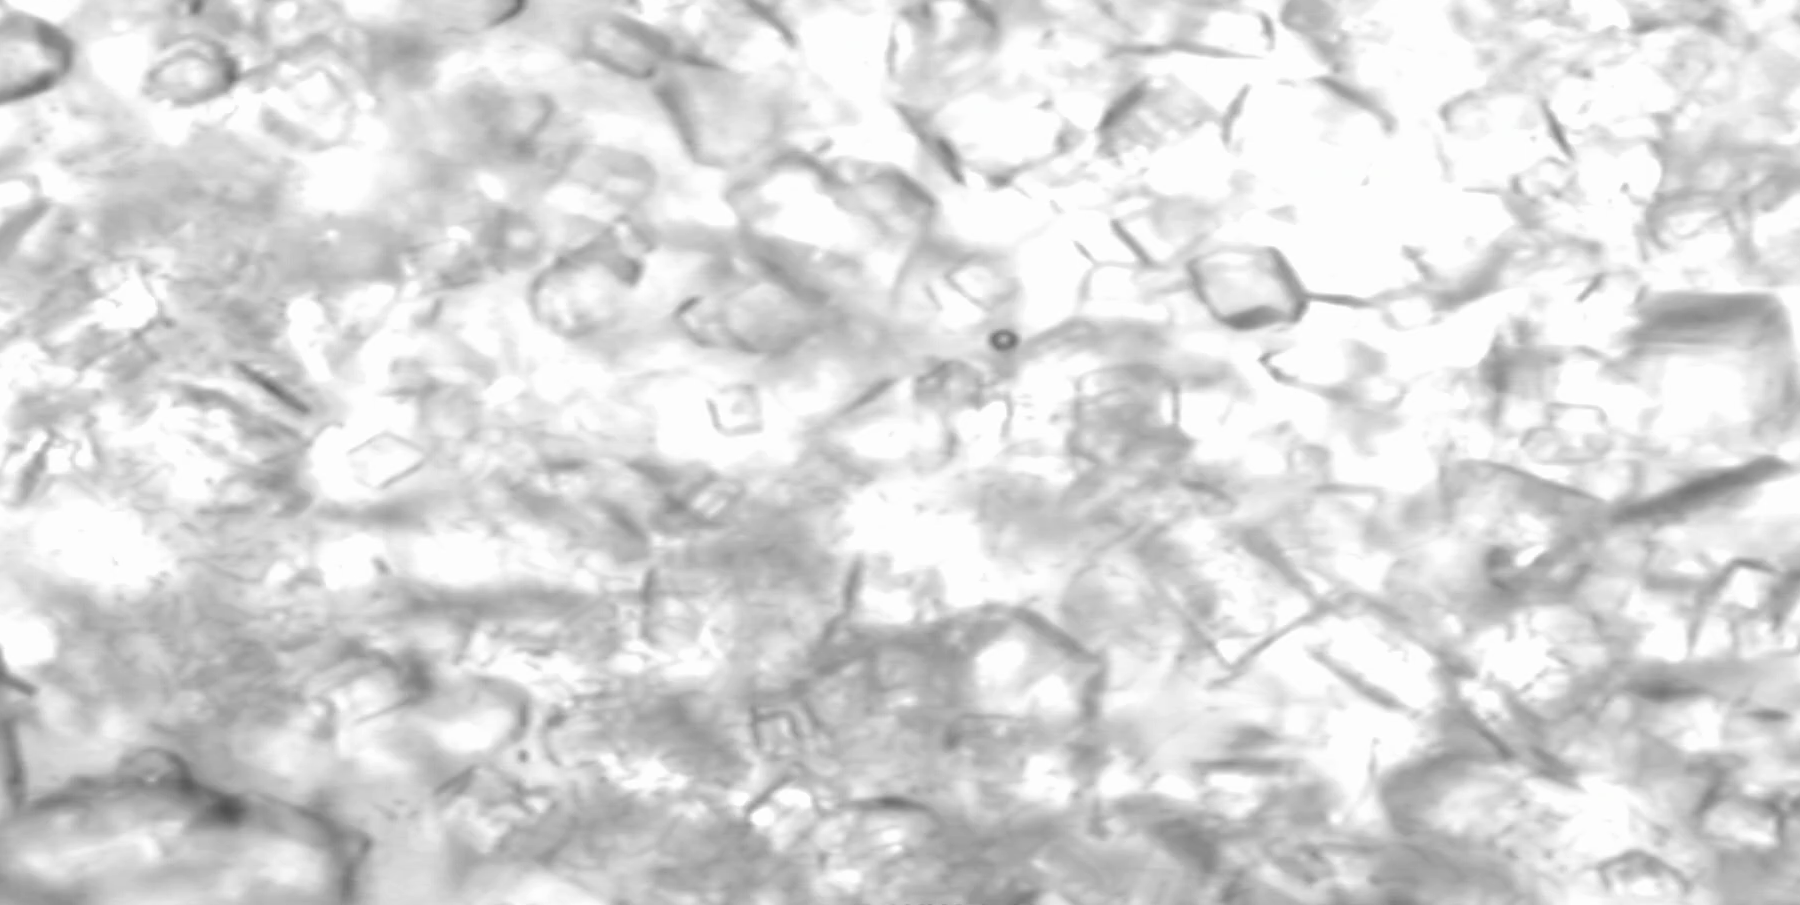
\includegraphics[width=\linewidth]{00_first_frame_cropped}
\caption{\textbf{What does the pipeline's input look like after frame conditioning?} Same frame after the two-step
crop removes both the DVR overlay and the analogue-aspect black bars ($1800 \times 905$~px $\approx 78$\,\% of the
raw frame area). The field is filled with sucrose crystals at varying defocus, with one crystal in focus near the
centre and progressively defocused crystals toward the periphery --- \emph{and no contamination sources left}.
Compare \secref{sec:empirical} for the quantitative impact of the crop on the measured Laplacian-variance $\alpha$
exponent.}\label{fig:frames-cropped}
\end{subfigure}
\caption{Raw and cropped first frame of the case-study video.}\label{fig:frames}
\end{figure}
